\scanpage{135}

Theorem of \handwritten{- - - - - -} (reported by Husemöller).

Let $A$ be a bialgebra over the field $k$, $A$ associative and unital for its two structures, ``cocomplete'' for its canonical comodule filtration (dual to the filtration by the powers of the augmentation ideal of the dual; more precisely, writing $\overset{n}{\otimes}A=\overset{n}{\otimes}A^{\handwritten{+}}+$ st\rlap{f}u\uline{f}f, whence via the m-th iterate\deleted{e} of the diagonal morphism, a map $A\handwritten{\longrightarrow}\overset{n}{\otimes}I^{\handwritten{+}}$, whose kernel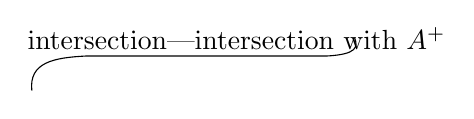
\begin{tikzpicture}[baseline=-.6ex,x=1cm,y=1cm]
\node[anchor=west,inner sep=0] at (0,.42) {\inserted{\handwritten{\unsure{intersection|intersection} with $A^{+}$}}};
\draw (.06,-.24) .. controls (.02,.12) and (.34,.18) .. (.75,.2) -- (3.8,.2) .. controls (4.2,.22) and (4.2,.32) .. (4.16,.43);
\end{tikzpicture} is $\mathrm{Filt}_{m}(A)$).\margin{\handwritten{this implies that there is an antipode ?}} (NB the cocompleteness hypothesis is satisfied for a coalgebra \inserted{with unit} in degrees $\handwritten{\geq}$ $0$ reduced to $k$ in degree\deleted{s} $0$, coassociative and counital, - apparently !). Let $M$ be an $A$-module, equipped with a counital diagonal homomorphism 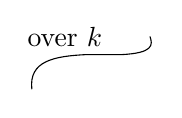
\begin{tikzpicture}[baseline=-.6ex,x=1cm,y=1cm]
\node[anchor=west,inner sep=0] at (0,.42) {\inserted{over $k$}};
\draw (.06,-.24) .. controls (.02,.12) and (.34,.18) .. (.75,.2) -- (1.2,.2) .. controls (1.6,.22) and (1.6,.32) .. (1.56,.43);
\end{tikzpicture} (perhaps not coassociative), $M\handwritten{\longrightarrow}M\otimes_{k}M$, which is $A$-linear,\margin{\figure{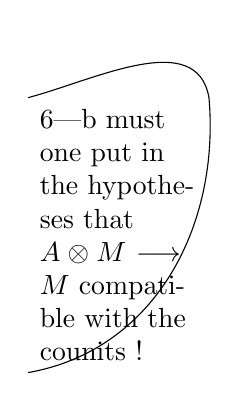
\begin{tikzpicture}
\node[text width=2cm,inner sep=4pt] (n) {\handwritten{\unsure{6|b} must one put in the hypotheses that $A\otimes M\longrightarrow M$ compatible with the counits !}};
\draw (n.north west) to[out=15,in=100] (n.north east) to[out=-85,in=10] (n.south west);
\end{tikzpicture}}}\inserted{\handwritten{(for the $A$-module structure on $M\unsure{\ominus|\otimes}M$ coming from $A\longrightarrow A\unsure{\otimes|\ominus}A$; it amounts to the same to say that $A\unsure{\ominus|\otimes}M\longrightarrow M$ compatible with diagonal map)}} Suppose further given a ``unit'' i.e. a homomorphism $k\handwritten{\longrightarrow}M$ which is a homomorphism of counital coalgebras, i.e. $\underset{M}{\mathrm{the}}$ image 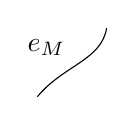
\begin{tikzpicture}[baseline=-.6ex,x=1cm,y=1cm]
\node[anchor=west,inner sep=0] at (0,.42) {\inserted{$e_M$}};
\draw (.13,-.2) .. controls (.46,.2) and (.94,.26) .. (1.01,.67);
\end{tikzpicture} of $1$ satisfies $\handwritten{\epsilon}_{M}(e_{M})=1$, $\handwritten{\Delta}_{M}(e_{M})=e_{M}\otimes e_{M}$. Suppose also $M$ cocomplete, and tha\unsure{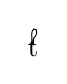
\begin{tikzpicture}[baseline=(e.base),x=1em,y=1em]
\node[inner sep=0] (e) at (0,0) {t};
\draw[line width=.35pt] (0,.1) .. controls (-.06,.28) and (-.08,.65) .. (.03,.67) .. controls (.2,.7) and (.14,.39) .. (.02,.34) -- (.01,.08);
\end{tikzpicture}}\deleted{one} the map $u\handwritten{\mapsto}u.e$ from $A$ to $M$ be injective. Then $M$ is a free $A$-module, 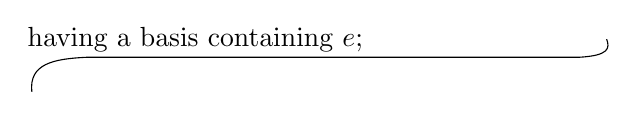
\begin{tikzpicture}[baseline=-.6ex,x=1cm,y=1cm]
\node[anchor=west,inner sep=0] at (0,.42) {\inserted{\handwritten{having a basis containing $e$;}}};
\draw (.06,-.24) .. controls (.02,.12) and (.34,.18) .. (.75,.2) -- (7.0,.2) .. controls (7.4,.22) and (7.4,.32) .. (7.36,.43);
\end{tikzpicture} more precisely, putting $\overset{\handwritten{-}}{M}=M\otimes_{A}k$, there exists a (noncanonical ...) isomorphism of $A$-modules $M\handwritten{\overset{\sim}{\unsure{\longleftarrow|\longleftrightarrow}}}A\otimes_{k}\overset{\handwritten{-}}{M}$\handwritten{, such that the diagram}
\margin{\handwritten{?}}
\handwritten{\diagram{\begin{tikzcd}[ampersand replacement=\&,column sep=small,row sep=small]
M \arrow[dr] \& \unsure{A|\mathcal{A}}\otimes_{k}\overline{M} \arrow[l,"\sim"'] \arrow[d] \\
\& \overline{M}
\end{tikzcd}}}
\handwritten{commutes, and that ...}

Example \handwritten{1}. Suppose the diagonal map of $A$ cocommutative. Then $A$ can be regarded as the hyperalgebra of a connected formal group 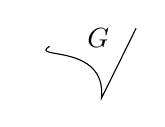
\begin{tikzpicture}[baseline=-.6ex,x=1cm,y=1cm]
\node[inner sep=0] at (.54,.52) {\inserted{$G$}};
\draw (-.08,.42) .. controls (-.35,.25) and (.65,.47) .. (.58,-.24) -- (1.02,.65);
\end{tikzpicture} over $k$. If $\handwritten{\Delta}_{M}$ is coassociative and cocommutative, $M$ too is formed of the distributions at the origin of a connected formal variety 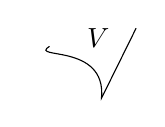
\begin{tikzpicture}[baseline=-.6ex,x=1cm,y=1cm]
\node[inner sep=0] at (.54,.52) {\inserted{$V$}};
\draw (-.08,.42) .. controls (-.35,.25) and (.65,.47) .. (.58,-.24) -- (1.02,.65);
\end{tikzpicture} over $k$, and the fact that $A$ acts on $M$ in such a way that the diagonal map is $A$-linear means that $G$ acts on $V$. One thus sees that if $u\handwritten{\unsure{\vdash|\mapsto}}\rlap{\(U\)}u.e$ 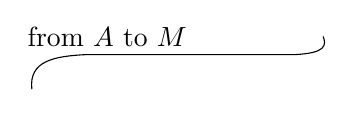
\begin{tikzpicture}[baseline=-.6ex,x=1cm,y=1cm]
\node[anchor=west,inner sep=0] at (0,.42) {\inserted{from $A$ to $M$}};
\draw (.06,-.24) .. controls (.02,.12) and (.34,.18) .. (.75,.2) -- (3.4,.2) .. controls (3.8,.22) and (3.8,.32) .. (3.76,.43);
\end{tikzpicture} is injective, i.e. if $g\handwritten{\mapsto}g.a$ ($a$ the \handwritten{``}center\handwritten{''} of $V$) from $G$ to $V$ is a monomorphism, then $M$ is free over $A$. In fact, one will find that $G$ acts freely on $V$ i.e.
% archive sheet number: 134
